\chapter{Testy}
\thispagestyle{chapterBeginStyle}

\section{15}
\label{15Test}
    \subsection{Wprowadzenie}
        Piętnastka (fr. taquin), znana również w Polsce o nazwie \textit{przesuwanka}, w zapisie często podawana przy pomocy liczbowego
        odpowiednika (15) jest grą w formie specyficznej
        układanki, której powstanie datuje się na koniec XIX wieku. Składa się ona z 
        15 klocków oraz ramki, pierwotnie drewnianej. Ramka zaprojektowana została specjalnie z myślą
        o pozostawieniu jednego wolnego miejsca, aby móc w łatwy sposób przesuwać klocki sąsiadujące \\
        z miejscem 
        pustym. Celem gry jest ułożenie klocków w określony sposób, najcześciej w porządku rosnącym czytając 
        od lewej do prawej rzędami, z określonego stanu początkowego. Częstym zabiegiem stosowanym przez 
        twórców ów układanki jest konwersja liczb na części obrazka, aby zachęcić do gry młodszych odbiorców.

        \begin{figure}[H]
            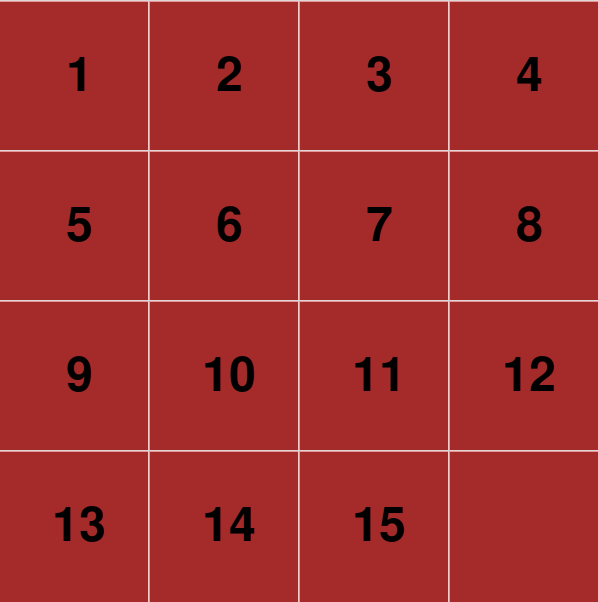
\includegraphics[scale=0.5]{15_ułożona}
            \centering
            \caption{Wygląd układanki piętnastki wygenerowany przy pomocy zaimplementowanej w ramach pracy warstwy graficznej}
        \end{figure}

        \begin{figure}[H]
            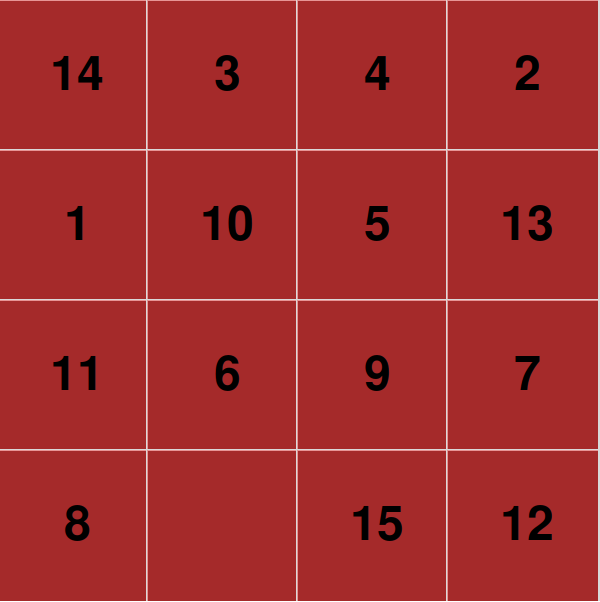
\includegraphics[scale=0.5]{15_losowe}
            \centering
            \caption{Losowa rozwiązywalna permutacja układanki}
        \end{figure}

    \subsection{Teoria}
        W 1878 roku amerykański wynalazca gier i zagadek (między innymi zagadek szachowych) \textbf{Samuel Loyd} ze względu na swój fach 
        nie przeszedł obojętnie koło piętnastki proponując ułożenie układu rosnącego z pozycji, która 
        od początkowej różniła się pozycjami jedynie dwóch klocków numerowanych odpowiednio 14 i 15 \cite{FifteenLoydProblem}.
        Problem ów stał się na tyle popularny, iż została wyznaczona nagroda 1000 dolarów dla osoby, której udałoby się 
        znaleźć prawidłowe rozwiązanie przygotowanego przez Pana Samuela problemu.

        Niemożliwość ułożenia problemu przez bardzo długi czas doprowadziła do pierwszych poważniejszych rozważań 
        nad z pozoru trywialną łamigówką. Efektem prac matematyków było parę zaskakujących wniosków, które ostatecznie doprowadziły 
        do udowodnienia, iż wyżej przedstawiona łamigłówka jest nierozwiązywalna.
        \begin{lemma}
            Nie wszystkie ustawienia początkowe piętnastki są możliwe do rozwiązania.\cite{Fifteen}
        \end{lemma}
        Wynika to z faktu, iż dla układanki o parzystych rozmiarach (w tym przypadku układanka jest rozmiarów 4x4)
        rozwiązywalne są jedynie ułożenia o parzystej liczbie inwersji. Zagadka Pana Loyd'a jest 
        ustawieniem nieparzystym jeśli chodzi o inwersje. Prowadzi to do następującego wniosku:
        \begin{corollary}
            Istnieje $\frac{16!}{2}=10 461 394 944 000$ rozwiązywalnych ustawień. 
        \end{corollary}
        Dodatkową ciekawostką istotną z perspektywy wykonywanych testów jest maksymalna liczba posunięć, którą należy wykonać, 
        aby z rozwiązywalnego stanu osiągnąć wcześniej wyznaczony cel. Mianem \textbf{boskiej liczby} w odniesieniu do przesuwanki
        określą się największą liczbę posunięć, którą trzeba osiągnąć, aby rozwiązać najtrudniejsze ułożeniem początkowe. Przy pomocy matematyki 
        naukowcy odnaleźli najtrudniejsze ustawienia oraz obliczyli ów liczbę, co zaprezentowano w następującym lemacie:
        \begin{lemma}
            \textbf{Boska liczba} dla 15-elementowej przesuwanki wynosi \textbf{80}. \cite{80Moves}
        \end{lemma}
        Oznacza to, iż maksymalna liczba kroków algorytmu w żadnym wypadku nie powinna przekroczyć liczby 80.

        W trakcie poniżej opisanego testu sprawdzono plany przesuwania odpowiednich klocków, aby w jak najmniejszej możliwej liczbie ruchów
        otrzymać odpowiedni stan końcowy, przy okazji sprawdzono osiągnięcia czasowe jak i porównano otrzymane wyniki z popularnymi herustykiami 
        spersonalizowanymi pod rozwiązywanie ów układanki.

    \subsection{Przykład}
        Na podstawie następującego przykładu zostanie przedstawiony schemat rozwiązywania układanki przez algorytm:
        \begin{figure}[H]
            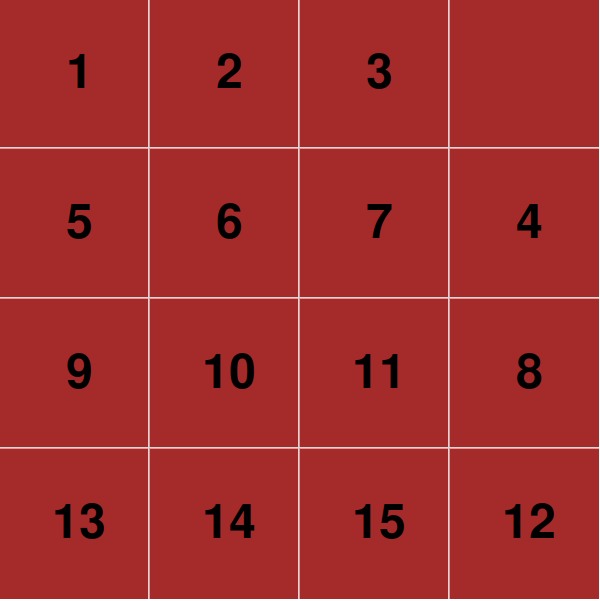
\includegraphics[scale=0.5]{15_przyklad}
            \centering
            \caption{Przykładowe startowe ułożenie przesuwanki}
            \label{Przyklad15}
        \end{figure}
        Algorytm buduje graf na podstawie jedynej zdefiniowanej w problemie akcji: przesuwania klocka. Robi to aż do momentu, gdy kafelki nie 
        będą ułożone w wczesniej zdefiniowanej kolejności. Dla zdefiniowanego powyżej przykładu w pierwszym kroku algorytm ma jedynie dwie możliwości 
        akcji aktywnych: zamiana klocka pustego z klockiem o numerze 3 lub klockiem o numerze 4. Na tej podstawie generuje kolejny poziom stanów. 
        Dla załączonego przykładu optymalnym rozwiązaniem jest odpowiednio zamiana pustego kafelka z kafelkami: 4,8,12, co zostało poprawnie 
        wyznaczone przez GRAPHPLAN. Poniżej przedstawiono zbiory akcji przeanalizowane przez algorytm w danym kroku jak i uproszczony graf planujący.

        \begin{figure}[H]
            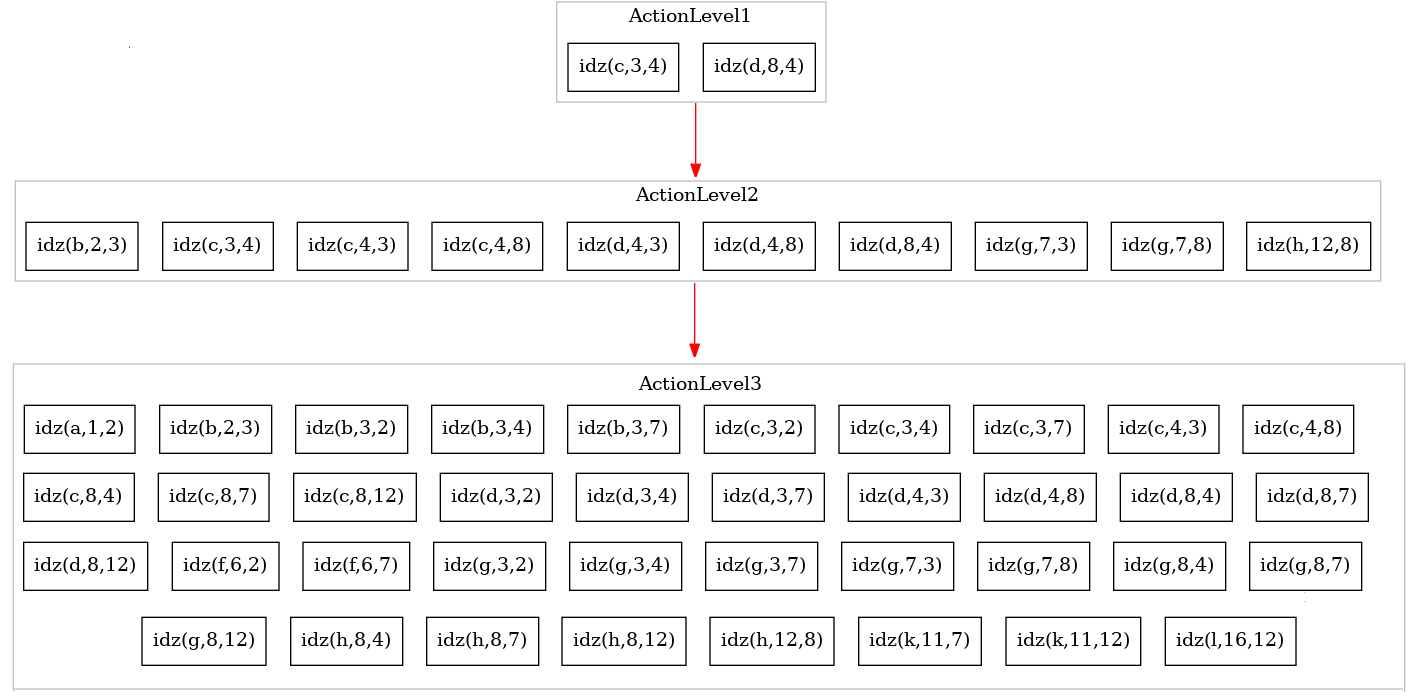
\includegraphics[scale=0.3]{15_zbiory_akcji}
            \centering
            \caption{Akcje rozpatrywane przez algorytm w danym kroku}
        \end{figure}

        \begin{figure}[H]
            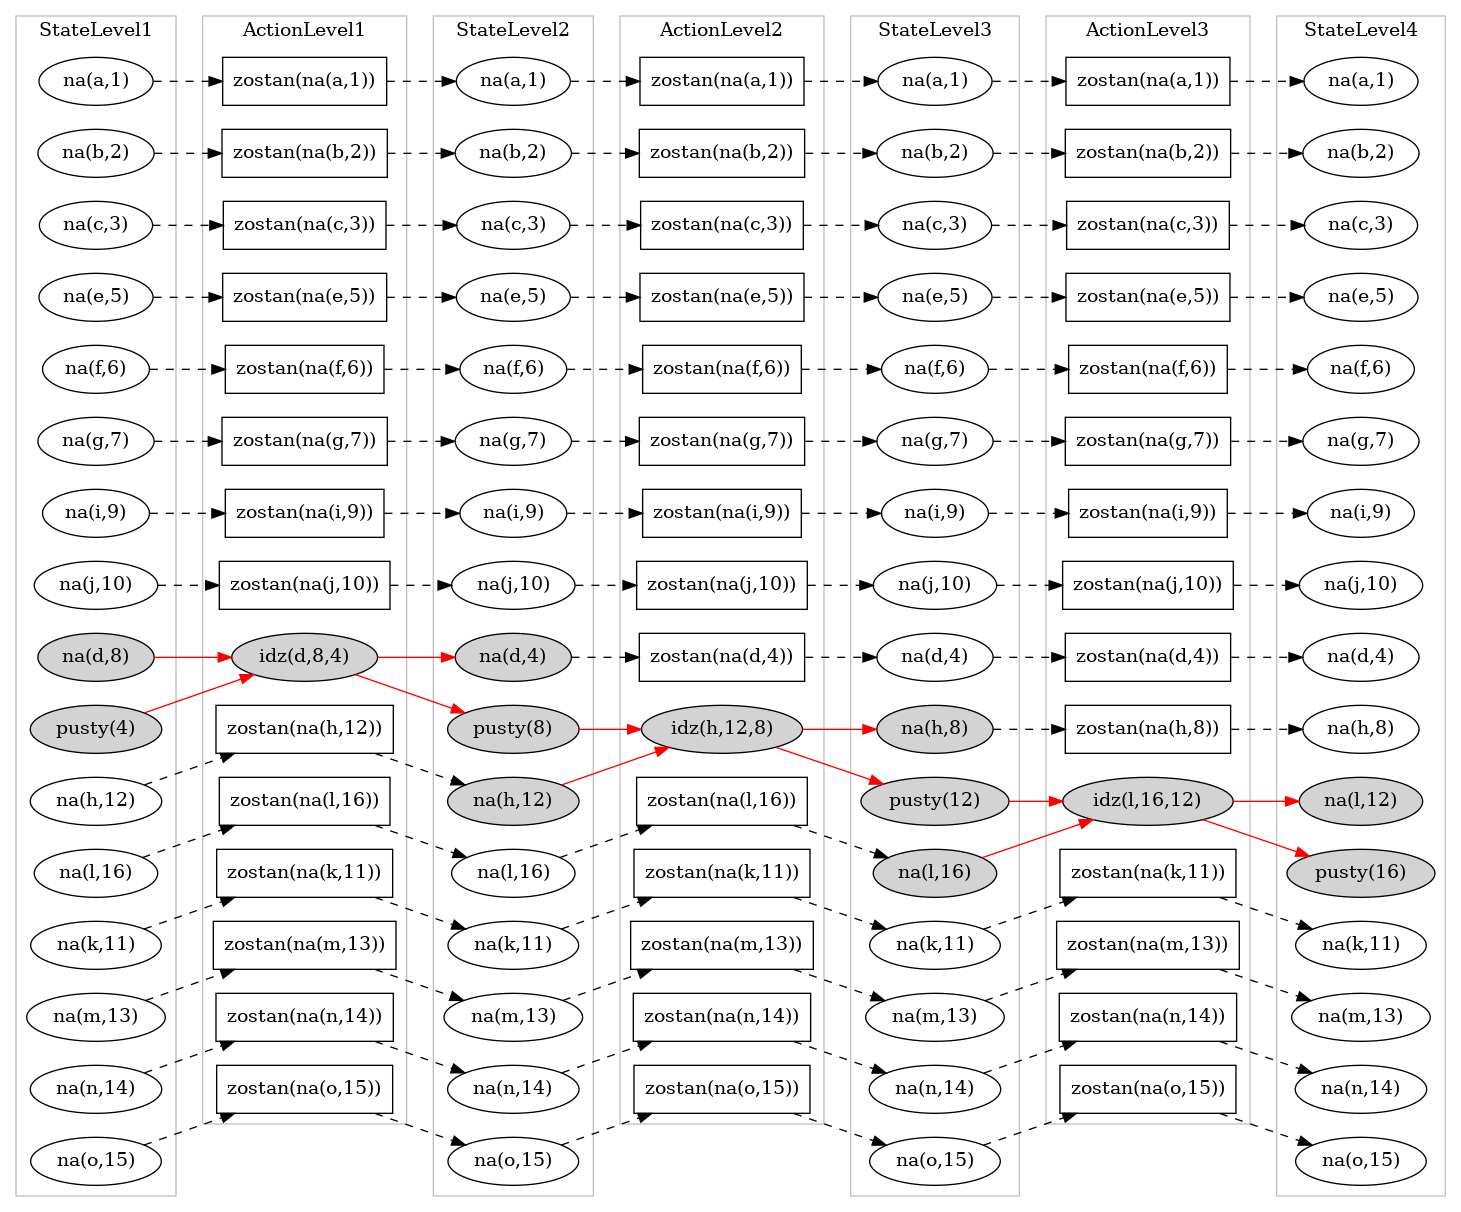
\includegraphics[scale=0.25]{15_graphplan}
            \centering
            \caption{Uproszczony graf planujący wygenerowany przez algorytm GRAPHPLAN przedstawiający stan każdego kafelka w danej warstwie. Węzły wypełnione 
            kolorem szarym obrazują stany, które są warunkami zajścia jak i efektami wykonywanej w danej warstwie akcji}
        \end{figure}

        \begin{figure}[H]
            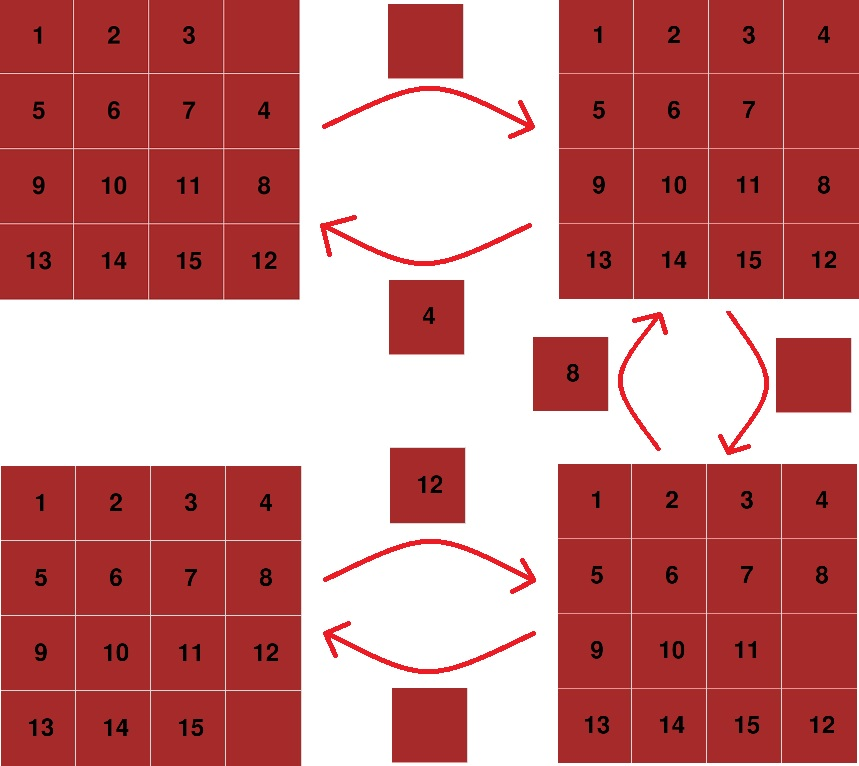
\includegraphics[scale=0.45]{15_zamiany}
            \centering
            \caption{Obrazowe rozwiązanie na podstawie wygenerowanego grafu}
        \end{figure}

    \subsection{Szczegóły implementacyjne}
    Ważnym jest, aby przedstawić omawiany świat zgodnie z wytycznymi ustalonymi przez język \textbf{STRIPS}. Z tego powodu należy dokładnie okreslić 
    każdą istniejącą relację, które zostaną użytę do definiowania stanów, akcji, warunków początkowych oraz celów. 
    Pierwszą określoną relacją będzie dwuargumentowa relacja na, której opis został już zawarty w sekcji \ref{RozdzialAkcje}.
    Relacja $na(A,B)$ informuje algorytm o tym, iż klocek $A$ znajduje się na pozycji $B$. Następnie należy zdefiniować każdy z klocków. 
    Wykorzystano do tego jednoargumentowy predykat o nazwie $robot(R)$. Ze względu na to, iż stałe w prologu oznaczane są przy pomocy 
    małych liter każdy z klocków zawiera swoje odzworowanie w literach. Poniższa ilustracja przedstawia proces mapowania klocka na literę:

    \begin{figure}[H]
        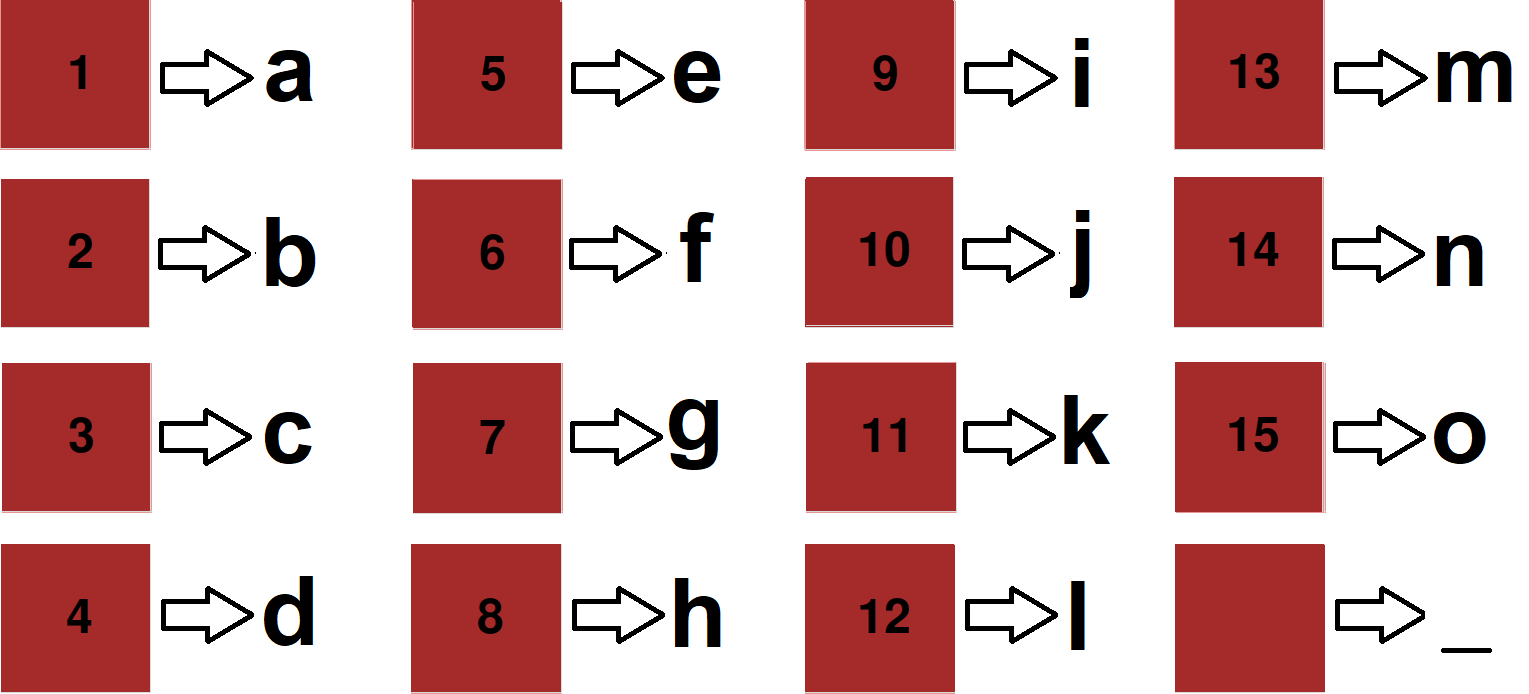
\includegraphics[scale=0.25]{mapowanieKlockow}
        \centering
        \caption{Przyporządkowywanie klockom odpowiednich liter}
    \end{figure}
    Ostatnie pole nie potrzebuje posiadać swojego odwzorowania w alfabecie, gdyż z nim związany jest predykat $pusty/1$, który informuje o tym, 
    iż dana pozycja jest pusta, \\
    lub z perspektywy algorytmu okupowana przez klocek o pustej sygnaturze. 

    W tym momencie należy wprowadzić rozróżnienie między klockiem a pozycją. Pozycje na planszy są stałe, numerowane rzędami od lewej do prawej,
    natomiast klocki mogą dynamicznie zmieniać swoje pozycję. Oznacza to tyle, iż numer klocka nie jest jednoznaczy \\ 
    z numerem pozycji. 
    Zrozumienie tego aspektu jest kluczowe, gdyż konwersja liczb na litery może prowadzić do zmieszania. 

    Jedyną akcją aktywną zdefiniowaną w ramach przesuwanki jest akcja $idz(R,A,B)$, która przesuwa klocek $R$ z pozycji $A$ na pozycję $B$.
    Zgodnie z wprowadzeniem literowych oznaczeń klocków, akcję $idz(a,4,8)$ należy rozumieć jako przesunięcie klocka z numerem 1 z pozycji 4 
    na pozycję 8 (czyli pionowo o jedną pozycję w dół w ostatniej kolumnie). Dla każdej akcji należy zdefiniować jej warunki zajścia jak i efekty.
    W przypadku przesuwanki dokonano tego przy pomocy predykatów $preconditions/2$ oraz $effects/2$. Poniżej znajdują się ich implementacje 
    w języku programowania PROLOG:
    \begin{listing}[H]
        \begin{minted}{prolog}
            %preconditions(+Action,-States)
            preconditions(zostan(P),[P]).

            preconditions(idz(R,A,B), [na(R,A), pusty(B)]) :-
                robot(R), 
                adjacent(A,B).
        \end{minted}
    \caption{Implementacja predykatu preconditions/2 dla przesuwanki}
    \end{listing}

    \begin{listing}[H]
        \begin{minted}{prolog}
            %effects(+Action,-States)
            effects(zostan(P),[P]).

            effects(idz(R,A,B), [na(R,B),pusty(A),~na(R,A),~pusty(B)]).
        \end{minted}
    \caption{Implementacja predykatu effects/2 dla przesuwanki}
    \end{listing}

    Należy zwrócić uwagę na fakt, iż każdy z predykatów występuje w dwóch wersjach, jedna odpowiada za akcje podtrzymującą, w skład której 
    zawsze wchodzi jeden warunek zajścia oraz jeden efekt, oraz drugą, która odpowiada akcji aktywnej. W przypadku predykatu $preconditions/2$
    wykorzystano relację $adjacent(A,B)$ która zachodzi w sytuacji, gdy pozycja $A$ sąsiaduje z pozycją $B$. Definicja sąsiedztwa jest identyczna 
    względem definicji wprowadzonej w \ref{DefinicjeSwiata}.

    \begin{listing}[H]
        \begin{minted}{prolog}
            %eadjacent(+From, +To)
            adjacent(A,B) :-
            n(A,B)
            ;
            n(B,A).
        \end{minted}
    \caption{Implementacja predykatu adjacent/2}
    \end{listing}
    
    Gdzie relacja $n(A,B)$ (n od angielskiego słowa neighbor oznaczajacego sąsiada)
    przedstawia relację sąsiedztwa pozycji $A$ z pozycją $B$. Poniżej przedstawiono rozkład relacji 
    sąsiedztwa dla każdej z pozycji wchodzącej w skład przesuwanki.

    \begin{listing}[H]
        \begin{minted}{prolog}
            n(1,2). n(1,5).
            n(2,1). n(2,6). n(2,3).
            n(3,2). n(3,7). n(3,4).
            n(4,3). n(4,8).
            n(5,1). n(5,6). n(5,9).
            n(6,5). n(6,2). n(6,7). n(6,10).
            n(7,6). n(7,3). n(7,8). n(7,11).
            n(8,7). n(8,4). n(8,12).
            n(9,5). n(9,10). n(9,13).
            n(10,9). n(10,6). n(10,11). n(10,14).
            n(11,10). n(11,7). n(11,12). n(11,15).
            n(12,11). n(12,8). n(12,16). 
            n(13,9). n(13,14).
            n(14,13). n(14,10). n(14,15).
            n(15,14). n(15,11). n(15,16).
            n(16,15). n(16,12).
        \end{minted}
    \caption{Modelowanie relacji sąsiedztwa}
    \end{listing}
    Ostatnim aspektem, bez którego wykonywanie działań w opiswyanym świecie byłoby niemożliwe, jest wprowadzenie stanów niespójnych, takich jak znajdowanie 
    się jednego bloczka na dwóch różnych pozycjach, bądź okupowanie jednej pozycji przez dwa różne klocki. Zostały to wykonane 
    przy pomocy predykatu $incosinstent/2$

    \begin{listing}[H]
        \begin{minted}{prolog}
            inconsistent(+State1,+State2)
            inconsistent(G,~G).
            inconsistent(~G,G).
            inconsistent(na(R,C1),na(R,C2)) :-
                C1 \== C2.
            
            inconsistent(na(_,C),pusty(C)).
            inconsistent(pusty(C),na(_,C)).
            inconsistent(na(R1,C),na(R2,C)) :-
                R1 \== R2.
        \end{minted}
    \caption{Implementacja predykatu inconsistent/2}
    \end{listing}

    Po zdefiniowaniu powyższych predykatów, algorytm jest gotowy do generowania odpowiednich planów mających za zadanie ułożenie 
    układanki z dowolnej rozwiązywalnej pozycji początkowej.
    \subsection{Wyniki}

    \textbf{UWAGA:} Testy czasowe zaprezentowane w poniższych tabelach tyczą się osiągów samego algorytmu. Oznacza to, iż na czas wykonywania prób
    wyłączone zostały wszystkie poboczne funkcjonalności takie jak generowanie grafu, czy prezentowanie rozwiązania w formie graficznej. 
    Wykonanie poniższych badań w aplikacji może skutkować innymi wynikami, zwykle dłuższymi. Ponadto testy czasowe obarczone są nieprawidłowościami 
    związanymi \\
    z działaniem innych, równoległych procesów w trakcie uruchamiania programu. Należy mieć to na uwadze przy potencjalnej 
    próbie odtwarzania badań.

    Z racji powyższego przedstawiono dodatkową metrykę wedle której zostanie dokonana ocena funkcjonalności algorytmu o nazwie \textbf{wnioskowania}.
    Jedno wnioskowanie jest utożsamiane z jednym podjęciem decyzji przez algorytm na dowolnym etapie realizacji. \\
    W kodach źródłowych (patrz Dodatek~\ref{plytaCD}) w katalogu \texttt{sources} znajduje się plik o nazwie \texttt{15\_tests.txt}, w którym 
    przedstawione są dokładne stany początkowe, dla których algorytm został uruchomiony, całkowity plan wygenerowany przez algorytm oraz 
    liczbę wnioskowań jak i wykorzystany czas dla każdego z przypadków. Ze względów objętościowych, \\
    w niniejszej pracy zostaną zamieszczone 
    jedyne najważniejsze informacje.

    \begin{table}[H]
        \centering
         \begin{tabular}{||c | c | c | c | c | c |} 
         \hline
         Przesunięcia & Test1 & Test2 & Test3 & Test4 & Test5 \\ [0.5ex] 
         \hline\hline
         1 & 0.009 & 0.009 & X & X & X \\ 
         \hline
         2 & 0.024 & 0.032 & 0.023 & 0.037 & X \\
         \hline
         3 &  0.048 & 0.177 & 0.177 & 0.048 & 0.178\\
         \hline
         4 &  0.35 & 0.757 & 0.334 & 0.357 & 0.776\\
         \hline
         5 &  1.315 & 1.181 & 1.188 & 1.188 & 1.197 \\
         \hline
         6 & 1.647 & 1.639 & 1.61 & 1.524 & 2.817\\ 
         \hline
         7 &  5.611 & 5.756 & 5.446 & 3.609 & 7.271\\
         \hline
         8 &  6.958 & 8.98 & 8.787 & 8.965 & 11.718 \\
         \hline
         9 &  13.471 & 9.54 & 13.911 & 8.859 & 9.041 \\
         \hline
         10 & 15.621 & 15.361 & 18.856 & 41.016 & 59.857 \\ [1ex]
         \hline
         \end{tabular}
         \caption{Przykładowe czasy, podawane w sekundach, dla wybranych przykładów zaokrąglone do trzeciej cyfry znaczącej dla 15}
    \end{table}
    Miejsce oznaczone lierą \texttt{X} oznaczają, iż dla danej liczby przesunięć nie istnieje możliwość wygenerowania większej liczby testów.
    \begin{table}[H]
        \centering
         \begin{tabular}{||c | c | c | c | c | c |} 
         \hline
         Przesunięcia & Test1 & Test2 & Test3 & Test4 & Test5 \\ [0.5ex] 
         \hline\hline
         1 & 1.002 & 1.001 & X & X & X \\ 
         \hline
         2 & 3.048 & 4.154 & 3.051 & 4.338 & X \\
         \hline
         3 & 6.565 & 24.755 & 24.703 & 6.58 & 24.879 \\
         \hline
         4 & 51.713 & 11748 874 & 5124 965 & 5189 118 & 11828 606 \\
         \hline
         5 & 179.368 & 178.311 & 181.251 & 181.122 & 181 \\
         \hline
         6 & 247.113 & 247.323 & 246.64 & 242.835 & 438.936\\ 
         \hline
         7 & 832.056 & 837.967 & 822.607 & 540.505 & 1115.938 \\
         \hline
         8 & 947.059 & 134 6.01 054 & 1256.889 & 1295.619 & 1722.644\\
         \hline
         9 & 1872.603 & 1401.642 & 1843.793 & 1385.176 & 1332.851\\
         \hline
         10 & 2250.796 & 4513.136  & 3029.235 & 5892.529 & 9592.842 \\ [1ex]
         \hline
         \end{tabular}
         \caption{Przykładowa liczba wnioskowań, podawana w setkach tysięcy, 
         zaokrąglona do trzech cyfr znaczących dla wybranych przykładów dla 15}
    \end{table}
    \begin{table}[H]
        \centering
         \begin{tabular}{||c | c | c|} 
         \hline
         Przesunięcia & Wnioskowania & Czas \\ [0.5ex] 
         \hline\hline
         1 & 1.001 & 0.009 \\ 
         \hline
         2 & 3.6 & 0.026 \\
         \hline
         3 & 17.5 & 0.126  \\
         \hline
         4 & 78.126 & 0.519  \\
         \hline
         5 & 180.211 & 1.214 \\
         \hline
         6 & 284.57 & 1.847 \\ 
         \hline
         7 & 829.814 & 5.539 \\
         \hline
         8 & 1313.644 & 9.082 \\
         \hline
         9 & 1567.213 & 10.953 \\
         \hline
         10 & 5055.707 & 34.255 \\ [1ex]
         \hline
         \end{tabular}
         \caption{Średnia liczba wnioskowania oraz czasów wykonania dla 15}
    \end{table}
    Przez \textit{przesunięcia} należy rozumieć liczbę przesunięć, którą należy wykonać, aby wrócić do początkowego stanu. Dla początkowych wartości 
    wskazanych w tabelach zostało to wyznaczone poprzez ręczne przestawienie kafelków o daną liczbę przesunięc oraz zapisanie otrzymanego stanu 
    przy użyciu nomenklatury opisanej w rozdziale definiujacym świat. Zgodnie z powyższym, analizując przykład \ref{Przyklad15} łatwo zauważyc, 
    iż wymaganą liczbą przesunięc, potrzebną do powrotu do wyjściowego stanu przesuwanki jest liczba \textbf{3} (co w dalszej części udało się 
    udowodnić konstruując odpowiedni plan).

    Analizując środowisko generowane przez przesuwankę naturalnym wnioskiem jest, iż maksymalnie jedna akcja może zostać wykonana dla danej 
    warstwy algorytmu. Wykorzystując dodatkową wiedzę o świecie, tylko i wyłącznie dla wskazanego przypadku zmodyfikowano algorytm w taki sposób,
    aby nie szukał alternatywnych rozwiązań we wskazanej warstwie, gdy odnajdzie już jedno oraz rozluźniono definicję relacji wzajemnie wykluczającej,
    wiedząc, iż równoległość nie ma większego wpływu na wygenerowane rozwiązania. Biorąc pod uwagę powyższą poprawkę odtworzono ponownie przygotowane
    testy. Dokładne wyniki zaprezentowane zostały w pliku \texttt{15\_tests\_modified.txt}, poniżej natomiast zamieszczono najważniejsze z nich:
    \begin{table}[H]
        \centering
         \begin{tabular}{||c | c | c | c | c | c |} 
         \hline
         Przesunięcia & Test1 & Test2 & Test3 & Test4 & Test5 \\ [0.5ex] 
         \hline\hline
         1 & 0.009 & 0.008 & X & X & X \\ 
         \hline
         2 & 0.023 & 0.027 & 0.023 & 0.025 & X \\
         \hline
         3 & 0.037  & 0.083 & 0.09  & 0.042 & 0.083\\
         \hline
         4 & 0.154 & 0.257 & 0.155 & 0.154 & 0.252\\
         \hline
         5 & 0.41 & 0.384 & 0.401 & 0.391 & 0.384 \\
         \hline
         6 & 0.503 & 0.501 & 0.503 & 0.488 & 0.783 \\ 
         \hline
         7 & 1.588 & 1.526 & 1.444 & 1.011 & 2.025\\
         \hline
         8 & 1.789 & 2.717 & 2.363 & 2.494 & 3.384 \\
         \hline
         9 & 3.954 & 2.594 & 2.734 & 3.087 & 2.05 \\
         \hline
         10 & 4.329 & 17.071 & 8.174 & 23.291 & 41.647 \\ [1ex]
         \hline
         \end{tabular}
         \caption{Przykładowe czasy dla wybranych przykładów, podawane w sekundach, zaokrąglone do trzeciej cyfry znaczącej dla modyfikacji algorytmu}
    \end{table}
    Miejsce oznaczone lierą \texttt{X} oznaczają, iż dla danej liczby przesunięć nie istnieje możliwość wygenerowania większej liczby testów.
    \begin{table}[H]
        \centering
         \begin{tabular}{||c | c | c | c | c | c |} 
         \hline
         Przesunięcia & Test1 & Test2 & Test3 & Test4 & Test5 \\ [0.5ex] 
         \hline\hline
         1 & 0.958 & 0.952 & X & X & X \\ 
         \hline
         2 & 2.527 & 3.065 & 2.533 & 3.077 & X \\
         \hline
         3 & 4.733 & 10.581 & 10.597 & 4.740 & 10.707 \\
         \hline
         4 & 33.138 & 19.205 & 19.491 & 19.018 & 33.482 \\
         \hline
         5 & 48.197 & 47.719 & 49.722 & 49.396 & 48.881\\
         \hline
         6 & 65.876 & 65.571 & 65.455 & 63.702 & 94.202\\ 
         \hline
         7 & 188.216 & 188.784 & 177.011 & 125.254 & 238.553 \\
         \hline
         8 & 216.004 & 343.949 & 281.063 & 307.151 & 444.794\\
         \hline
         9 & 471.810 & 310.744 & 313.831 & 311.831 & 246.464\\
         \hline
         10 & 517.519 & 2604.262 & 1014.235 & 3063.34 & 5781.37 \\ [1ex]
         \hline
         \end{tabular}
         \caption{Przykładowa liczba wnioskowań, podawana w setkach tysięcy, 
         zaokrąglona do trzech cyfr znaczących dla wybranych przykładów dla modyfikacji algorytmu}
    \end{table}
    \begin{table}[H]
        \centering
         \begin{tabular}{||c | c | c|} 
         \hline
         Przesunięcia & Wnioskowania & Czas \\ [0.5ex] 
         \hline\hline
         1 & 0.952 & 0.009 \\ 
         \hline
         2 & 2.8 & 0.024 \\
         \hline
         3 & 8.271 & 0.067 \\
         \hline
         4 & 24.867 &  0.194 \\
         \hline
         5 & 48.783 & 0.394 \\
         \hline
         6 & 70.961 & 0.557 \\ 
         \hline
         7 & 183.564 & 1.519 \\
         \hline
         8 & 318.592 & 2.549 \\
         \hline
         9 & 330.954 & 2.884 \\
         \hline
         10 & 2596.204 & 18.902 \\ [1ex]
         \hline
         \end{tabular}
         \caption{Średnia liczba wnioskowania oraz czasów wykonania dla modyfikacji algorytmu}
    \end{table}


    Wykres zestawiający osiągi obu podejść:

    \begin{figure}[H]
        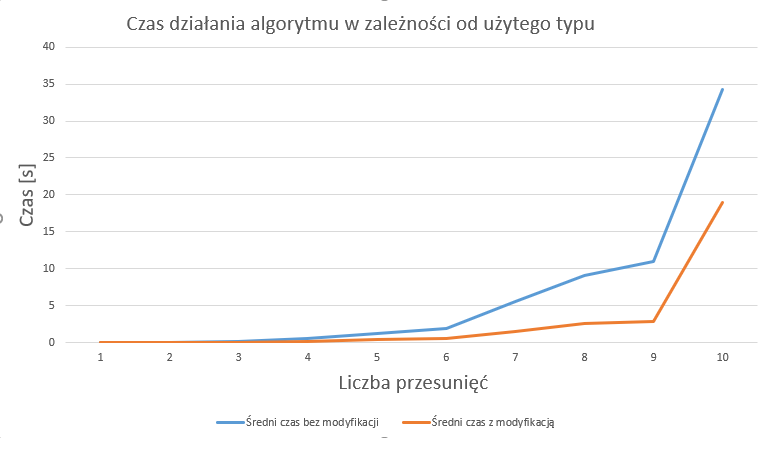
\includegraphics[scale=0.8]{Wykres15Czas}
        \centering
        \caption{Porównanie czasów dla piętnastki}
        \label{CargoObrazek2}
    \end{figure}
    \begin{figure}[H]
        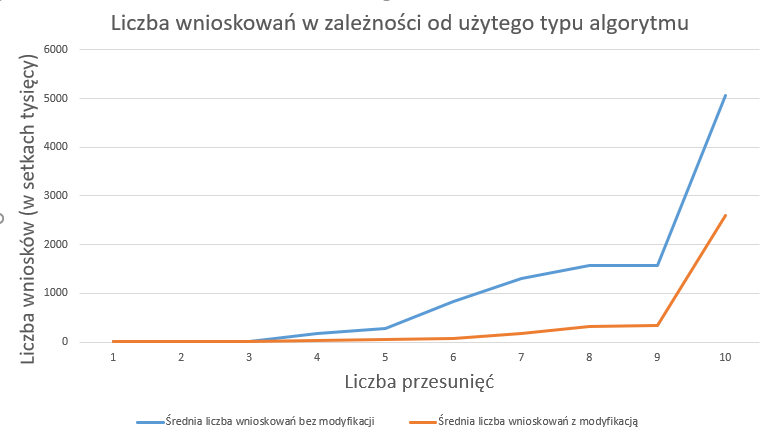
\includegraphics[scale=0.8]{Wykres15Wnioski}
        \centering
        \caption{Porównanie wnioskowań dla piętnastki}
        \label{CargoObrazek2}
    \end{figure}


    \subsection{Młodsza siostra- ósemka}
        Ósemka jest inną formą przesuwanki- zamiast tradycyjnego ułożenia 15 klocków w kształcie kwadratu 4 na 4 z jednym wolnym miejscem, ósemka 
        składa się z osmiu klocków, które ułożone zostały w kształcie kwadratu 3 na 3. Powoduje to zmniejszenie dziedziny, a co za tym idzie- 
        łatwiejsze i szybsze układanie. Dla ósemki wszystkie definicje i własności są identyczne jak dla pietnastki, z drobnym wyjątkiem- dla 
        układanki o osmiu klockach i jednym pustym polu \textbf{boska liczba} wynosi nie 80 a 31\cite{Eight} liczba możliwych ułożeń wynosi 
        \begin{equation}
            \frac{8!}{2} = 181440
        \end{equation} 
        oraz lekkiej modyfikacji uległ predkyat $n/2$
    \subsection{Wyniki dla 8}
        Wersja ze zmniejszoną liczbą klocków została poddana identycznym testom jak piętnastka. Poniżej przedstawione zostały rezultaty 
        przeprowadzonych badania:
        \begin{listing}[H]
            \begin{minted}{prolog}
                n(1,2). n(1,4).
                n(2,1). n(2,3). n(2,5).
                n(3,2). n(3,6).
                n(4,1). n(4,5). n(4,7).
                n(5,4). n(5,6). n(5,2). n(5,8).
                n(6,5). n(6,3). n(6,9).
                n(7,4). n(7,8).
                n(8,7). n(8,5). n(8,9).
                n(9,8). n(9,6).
            \end{minted}
        \caption{Modelowanie relacji sąsiedztwa dla ósemki}
        \end{listing}
        \begin{table}[H]
            \centering
             \begin{tabular}{||c | c | c | c | c | c |} 
             \hline
             Przesunięcia & Test1 & Test2 & Test3 & Test4 & Test5 \\ [0.5ex] 
             \hline\hline
             1 & 0.003 & 0.003 & --- & --- & --- \\ 
             \hline
             2 & 0.022 & 0.025 & 0.009 & 0.012 & ---   \\
             \hline
             3 & 0.067 & 0.068 & 0.069 & 0.7 & 0.068  \\
             \hline
             4 & 0.135 & 0.135 & 0.141 & 0.136 & 0.383 \\
             \hline
             5 & 0.554 & 0.554 & 0.538 & 0.554 & 0.549 \\
             \hline
             6 & 0.684 & 0.701 & 0.719 & 1.14 & 0.702 \\ 
             \hline
             7 & 1.495 & 1.386 & 1.888 & 1.724 & 1.511  \\
             \hline
             8 & 1.621 & 1.625 & 1.888 & 1.724 & 1.511  \\
             \hline
             9 & 3.207 & 3.582 & 7.568 & 4.056 & 3.593  \\
             \hline
             10 & 5.159 & 4.208 & 6.065 & 6.528 & 14.906  \\ [1ex]
             \hline
             \end{tabular}
             \caption{Przykładowe czasy, podawane w sekundach, dla wybranych przykładów z ósemki}
        \end{table}
    
        \begin{table}[H]
            \centering
             \begin{tabular}{||c | c | c | c | c | c |} 
             \hline
             Przesunięcia & Test1 & Test2 & Test3 & Test4 & Test5 \\ [0.5ex] 
             \hline\hline
             1 & 0.321 & 0.321 & X & X & X \\ 
             \hline
             2 & 2.607 & 2.617 & 1.045 & 1.045 & X \\
             \hline
             3 & 8.111 & 8.13 & 8.228 & 8.183 & 8.183 \\
             \hline
             4 & 17.026 & 16.847 & 17.005 & 17.017 & 51.037 \\
             \hline
             5 & 73.589 & 72.195 & 72.494 & 70.408 & 72.914  \\
             \hline
             6 & 91.771 & 93.703 & 95.256 & 149.296 & 933.376 \\ 
             \hline
             7 & 208.006 & 173.973 & 265.5 & 234.793 & 211.315 \\
             \hline
             8 & 219.776 & 221.114 & 335.280 & 465.878 & 572.589 \\
             \hline
             9 & 449.784 & 498.638 & 1118.575 & 547.934 & 493.647 \\
             \hline
             10 & 772.697 & 604.193 & 891.039 & 969.741 & 2279.220 \\ [1ex]
             \hline
             \end{tabular}
             \caption{Przykładowa liczba wnioskowań dla wybranych przykładów w 8-elementowej układance}
        \end{table}
    
        \begin{table}[H]
            \centering
             \begin{tabular}{||c | c | c|} 
             \hline
             Przesunięcia & Wnioskowania & Czas \\ [0.5ex] 
             \hline\hline
             1 & 0.321 & 0.003 \\ 
             \hline
             2 & 1.829 & 0.17 \\
             \hline
             3 & 8.167 &  0.068 \\
             \hline
             4 & 23.786 &  0.186 \\
             \hline
             5 & 72.172 &  0.546\\
             \hline
             6 & 104.673 &  0.789\\ 
             \hline
             7 & 218.717 &  1.601\\
             \hline
             8 & 362.927 &  2.578\\
             \hline
             9 & 621.715 &  4.401\\
             \hline
             10 & 1103.378 & 7.373\\ [1ex]
             \hline
             \end{tabular}
             \caption{Średnia liczba wnioskowania oraz czasów wykonania dla ósemki}
        \end{table}

        Podobną modyfikację można wykonać dla pomniejszonego wariantu łamigłówki, z bardzo zbliżonym efektem, co pokazuję następujące badania:
        \begin{table}[H]
            \centering
             \begin{tabular}{||c | c | c|} 
             \hline
             Przesunięcia & Wnioskowania & Czas \\ [0.5ex] 
             \hline\hline
             1 & 0.29 & 0.003 \\ 
             \hline
             2 & 1.216 & 0.011 \\
             \hline
             3 & 3.878 & 0.035 \\
             \hline
             4 & 8.592 & 0.062 \\
             \hline
             5 & 20.945 & 0.168 \\
             \hline
             6 & 31.115 & 0.247 \\ 
             \hline
             7 & 96.639 & 0.659 \\
             \hline
             8 & 166.713 & 1.097 \\
             \hline
             9 & 427.269 & 2.941 \\
             \hline
             10 & 885.724 & 5.504 \\ [1ex]
             \hline
             \end{tabular}
             \caption{Średnia liczba wnioskowania oraz czasów wykonania dla zmodyfikowanej ósemki}
        \end{table}

        \begin{figure}[H]
            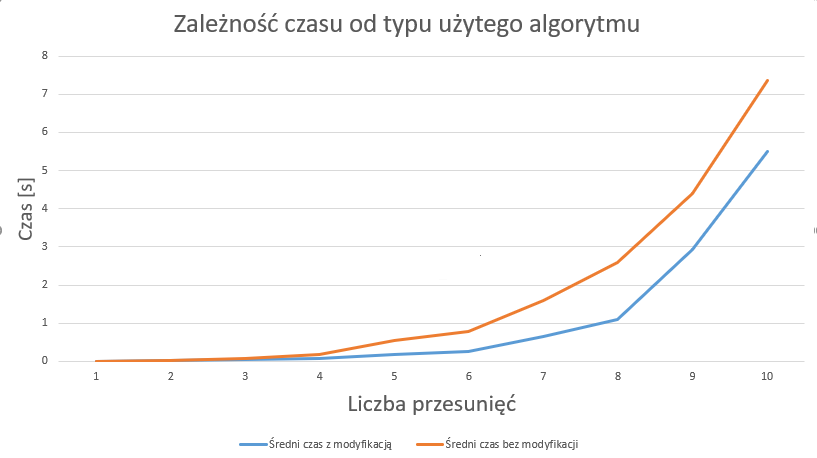
\includegraphics[scale=0.8]{WykresCzas8}
            \centering
            \caption{Porównanie czasów dla ósemki}
        \end{figure}
        \begin{figure}[H]
            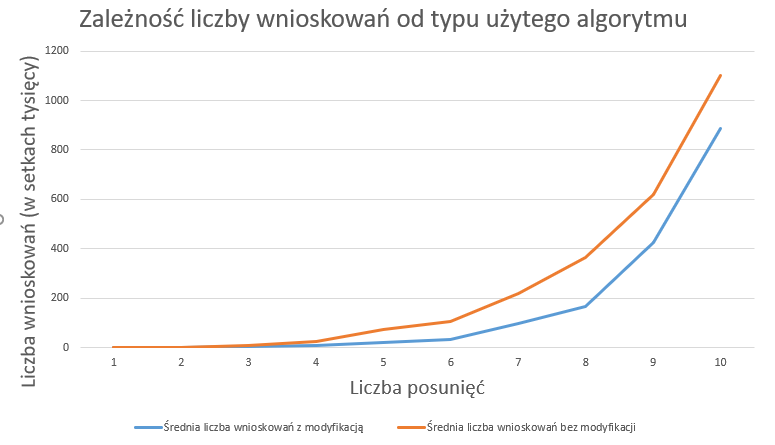
\includegraphics[scale=0.8]{WykresWnioskowania8}
            \centering
            \caption{Porównanie wnioskowań dla ósemki}
        \end{figure}



    \subsection{Wnioski}
        Dla zdefiniowanego świata GRAPHPLAN poprawnie generuje plany. Empiryczne sprawdzenie wykazało, iż faktycznie są to plany optymalne. Ponadto 
        dla mniejszych przykladów generowanie planów trwa stosunkowo krótko, jednakże w sytuacji, gdy dojdzie do spłaszczenia grafu planującego, 
        co dla przesuwanki z 15 klockami dzieje się w okolicach 10 iteracji, wydajność algorytmu znacznie spada. Podobne efekty zostały 
        zaobserwowane dla układanki z 8 klockami. Wprowadzenie modyfikacji odnośnie równoległości doprowadziło do poprawy otrzymanych rezultatów.
        Porównanie z specjalnie utworzonymi na potrzeby układanki heurstykami pokazały, iż są one 
        znacząco szybsze niż algorytm planujący, jednakże duża zaletą GRAPHPLAN'u jest uniwersalność, gdyż można go stosować do innych problemów.
        Heurstyki natomiast rozwiązują problem jedynie dla danej układanki.
\section{CargoBot}
\label{CargoBotTest}
    \subsection{Wprowadzenie}
        \textbf{CargoBOT} (Twórcy: \textbf{Two Lives Left}) jest grą dostępną w platformie dystrybucji cyfrowej o nazwie \textbf{App Store},
        która znajduje się na urządzeniach wyprodukowanych przez firmę \textbf{Apple}. 
        Głównym celem gry jest przestawienie skrzynek z pozycji początkowej na przedstawioną 
        pozycję końcową przy użyciu ramienia, które może poruszać się w prawo, w lewo oraz opuszczać na dół. Podczas opuszczania, jeśli w 
        ramieniu znajduje się skrzynka to zostanie opuszczona, natomiast jeśli ramię nie trzyma żadnej skrzynki podniesie pierwszą na jaką 
        natrafi. Przypatrując się bliżej powyższemu opisowi, nie sposób nie zauważyć połączenia przedstawionego świata z językiem opisowym 
        STRIPS. Z tego powodu kolejnym testem możliwości GRAPHPLAN'u będzie rozwiązywanie zagadek przedstawionych przez aplikację \textbf{CargoBOT}.
        \textbf{UWAGA: } W grze CargoBOT celem użytkownika jest zaprojektowanie algorytmu przy pomocy specjalnego panelu do rozwiązywania łamigłówki.
        Ze względu na to, iż celem testu jest przedstawienie optymalnego planu otrzymującego stan końcowy ze stanu początkowego, wynik algorytmu 
        nie będzie bezpośrednio rozwiązaniem korzystającym z nomenklatury aplikacji.
    \subsection{Szczegóły implementacyjne}
    Przed rozpoczęciem generowania planu, podobnie jak w przypadku poprzednich testów, należy rozpocząć modelowanie świata zgodnie z wytycznymi 
    języka opisu STRIPS. Pierwsze zaimplementowane predykaty to $block/1$ oraz $place/1$. Fakt $block(a)$ oznacza skrzynkę z etykietą a, natomiast 
    $place(1)$ oznacza miejsce z etykietą 1. Ze względu na ograniczenia językowe, każdy z bloków oraz każde z miejsc musi mieć unikatową etykietę. 
    Spowoduje to, iż nie wszystkie łamigłówki z aplikacji będą możliwe do reprodukcji ze względu na to, \\
    że paczki w grze rozróżnialne są od siebie 
    jedynie ze względu na \textit{kolor}. Dodatkowo przez pojęcie miejsca rozumie się przestrzeń, na której może leżeć bloczek. Miejsca można
    wyobrażać sobie jakie półki, bądź platformy, które są od siebie odzielone pewną przeszkodą bądź wolną przestrzenią. Przykład \ref{CargoObrazek1}
    przedstawia reprezetancję miejsc w formie czarnych, poziomych kresek. 
    
    To co odróżnia opis świata dla aplikacji CargoBOT od przesuwanki to fakt, iż liczba skrzynek oraz platform może zmieniać się dynamicznie w zależności 
    od świata. Z tego powodu za każdym razem należy upewnić się, iż wszystkie obiekty zostały opisane w języku algorytmu przy pomocy wyżej przedstawionych 
    predykatów. 

    Jedyną akcją rozpatrywaną jest przesuwanie przy użyciu ramienia skrzynki z jednej platformy na drugą. Akcja ta będzie nazwana identycznie jak w 
    przypadku przesuwanki przy pomocy czasownika $idz$. Trójargumentowa relacja $idz(S,A,B)$ oznacza przesunięcie skrzynki $S$ z platformy $A$
    na platformę $B$. Poniżej przedstawiono implementację warunków zajścia jak i efektów przedstawionej akcji:

    \begin{listing}[H]
        \begin{minted}{prolog}
            %preconditions(+Action,-States)
            preconditions(zostan(P),[P]).

            preconditions(idz(Block,From,To), 
            [pusty(Block),pusty(To),na(Block,From)]) :-
                block(Block),
                object(To),
                To \==Block,
                object(From),
                From \==To,
                Block \== From.
        \end{minted}
    \caption{Implementacja predykatu preconditions/2 dla CargoBOT'a}
    \end{listing}

    \begin{listing}[H]
        \begin{minted}{prolog}
            %effects(+Action,-States)
            effects(zostan(P),[P]).

            effects(idz(X,From,To),[na(X,To),pusty(From),~na(X,From),~pusty(To)]).
        \end{minted}
    \caption{Implementacja predykatu effects/2 CargoBOT'a}
    \end{listing}
    W przypadku akcji przesunięcia warto zaznaczyć, iż może zaistnieć sytuacja, w której najlepszą drogą uzyskania stanu końcowego jest 
    umieszczenie jednej paczki na drugiej. Stąd znane już czytelnikowi predykaty $na/2$ oraz $pusty/1$ w tym przypadku będą się odnosić do skrzynek, 
    ale również do platform. Przyglądając się ciału predykatu $preconditions/2$ należy zauważyć, iż dochodzi do sprawdzenia, czy 
    to co znajduje się w zmiennej $Block$ jest typu block, oraz czy zmienne $From$ oraz $To$ są obiektami świata. 
    Predykat $object/1$ realizowany jest w następujący sposób:

    \begin{listing}[H]
        \begin{minted}{prolog}
            %object(+Variable)
            object(X) :-
                place(X)
                ;
                block(X).
        \end{minted}
    \caption{Implementacja predykatu object/1}
    \end{listing}

    Zgodnie z definicją obiektu, platformy również są obiektami.

    Dodatkowe sprawdzenia wykonywane w ramach warunków zajścią mają za zadanie uniknięcie sytuacji, w której planer chciałbym przenieść skrzynkę 
    na samą siebie.
    Implementacja relacji wzajemnie wykluczającej odbyła się w sposób identyczny jak dla 15. Użyty został predykat $inconsistent/2$.
    W powyższy sposób ukończono implementację świata z gry CargoBOT.

    \subsection{Przykład}  
    Celem algorytmu będzie rozwiązanie następującego problemu:
    \begin{figure}[H]
        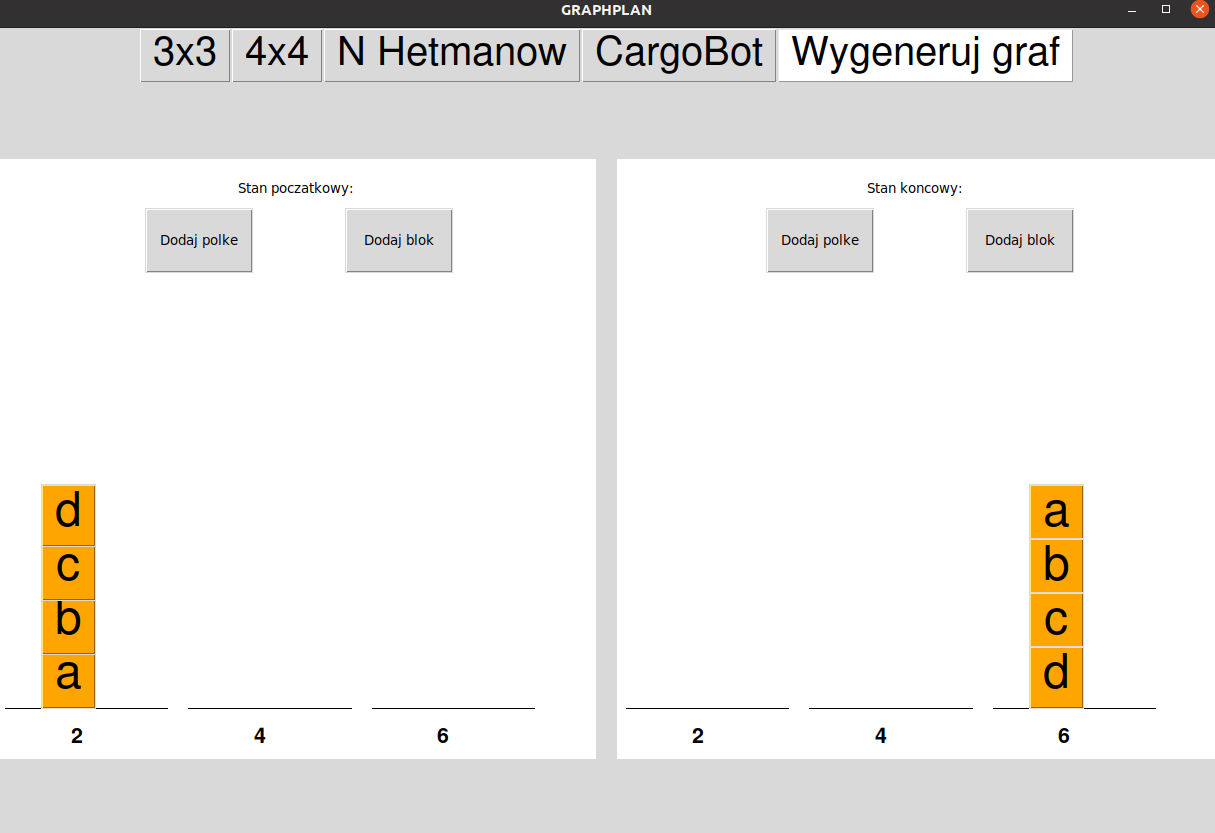
\includegraphics[scale=0.35]{cargo_przyklad1}
        \centering
        \caption{Reprezentacja łamigłówki w aplikacji}
        \label{CargoObrazek1}
    \end{figure}
    Po naciśnięciu przycisku \textit{Wygeneruj graf} widok zmienia się w następujący sposób:
    \begin{figure}[H]
        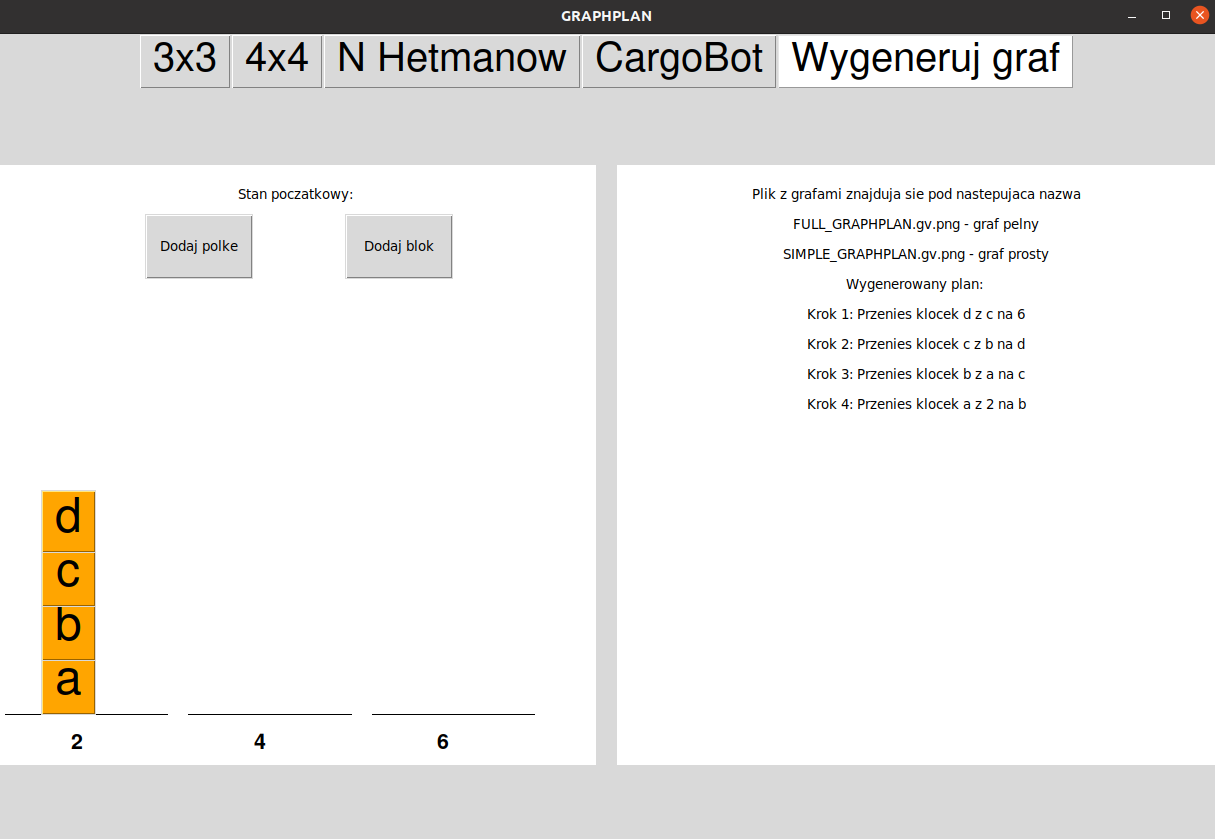
\includegraphics[scale=0.4]{cargo_przyklad2}
        \centering
        \caption{Rozwiązanie w formie listy kroków zaprezentowane w aplikacji}
        \label{CargoObrazek2}
    \end{figure}
    Poniżej zamieszczono wygenerowany graf prosty dla rozpatrywanego przypadku:
    \begin{figure}[H]
        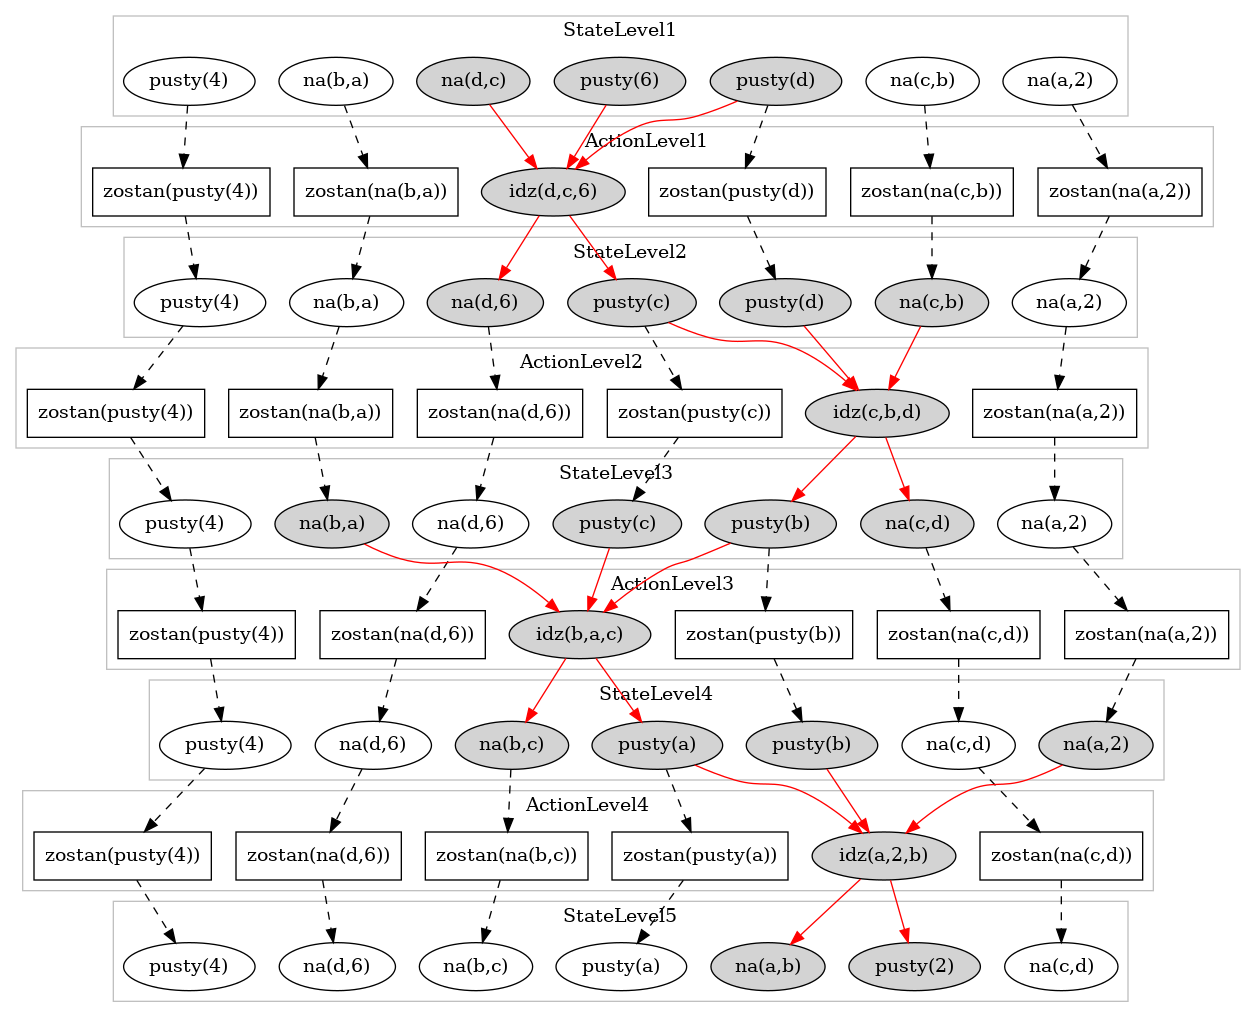
\includegraphics[scale=0.25]{cargo_przyklad1_graf}
        \centering
        \caption{Reprezentacja łamigłówki w aplikacji}
        \label{CargoObrazek3}
    \end{figure}

    \subsection{Wyniki}
    \begin{table}[H]
        \centering
         \begin{tabular}{||c | c | c| c |} 
         \hline
         Nazwa łamigłówki & Liczba kroków & Wnioskowania & Czas \\ [0.5ex] 
         \hline\hline
         Cargo101 & 1 & 4 461 & 0.001 \\ 
         \hline
         Transporter & 1 & 14 4661 & 0.001 \\
         \hline
         Re-curses & 4 & 611 018 & 0.06 \\
         \hline
         Inverter & 4 & 6 705 348 & 0.585 \\
         \hline
         Double Flip & 7 & 49 091 704 & 2.983 \\
         \hline
         Shuffle Sort & 6 & 10 285 196 & 0.909 \\ 
         \hline
         Go to the distance & 4 & 377 831 393 & 35.487 \\
         \hline
         Color sort & 6 & 10 431 817 & 0.915 \\ [1ex]
         \hline
         \end{tabular}
         \caption{Rozwiązania dla łamigłówek z aplikacji}
    \end{table}
    Zgodnie z wczesniejszymi założeniami, wartości w kolumnie \textbf{wnioskowania} podawane są w setkach tysięcy, natomiast 
    w kolumnie \textbf{czas}- w sekundach.



    \subsection{Wnioski}
    Zgodnie z oczekiwaniami, zaprezentowane łamigłówki zostały rozwiązane przez GRAPHPLAN z wykorzystaniem najmniejszej liczby kroków. 
    Dodatkowe zadanie pokazało również siłę wykorzystania częściowego porządku układając dwie częsci łamigłówki równoczesnie. Łatwo zauważyć,
    iż ze względu na strukturę GRAPHPLAN'u dodanie elementów do świata znacząco wpływa na tempo rozwiązywania zadań, mimo faktu, iż cel jak i warunki 
    początkowe nie zmieniły się znacząco między łamigłówkami. 
\section{Plany z równoległością}
    \subsection{Wprowadzenie}
    Poprzednie przykłady operowały na sytuacjach, dla których optymalny plan sprowadzał się do wykonywania jednej czynności w danym kroku. Własnośc ta
    może zostać użytak jako zaleta, co można było zaobserwować w przypadku przesuwanki. 
    Istnieje jednak wiele sytuacji, w których równoległe wykonywanie akcji jest wymagane, aby 
    osiągnąć cel w jak najmniejszej liczbie kroków.
    \subsection{Przykłady}
    Pierwszy przykład ulega ułożeniu planu dla następujących warunków:
    \begin{figure}[H]
        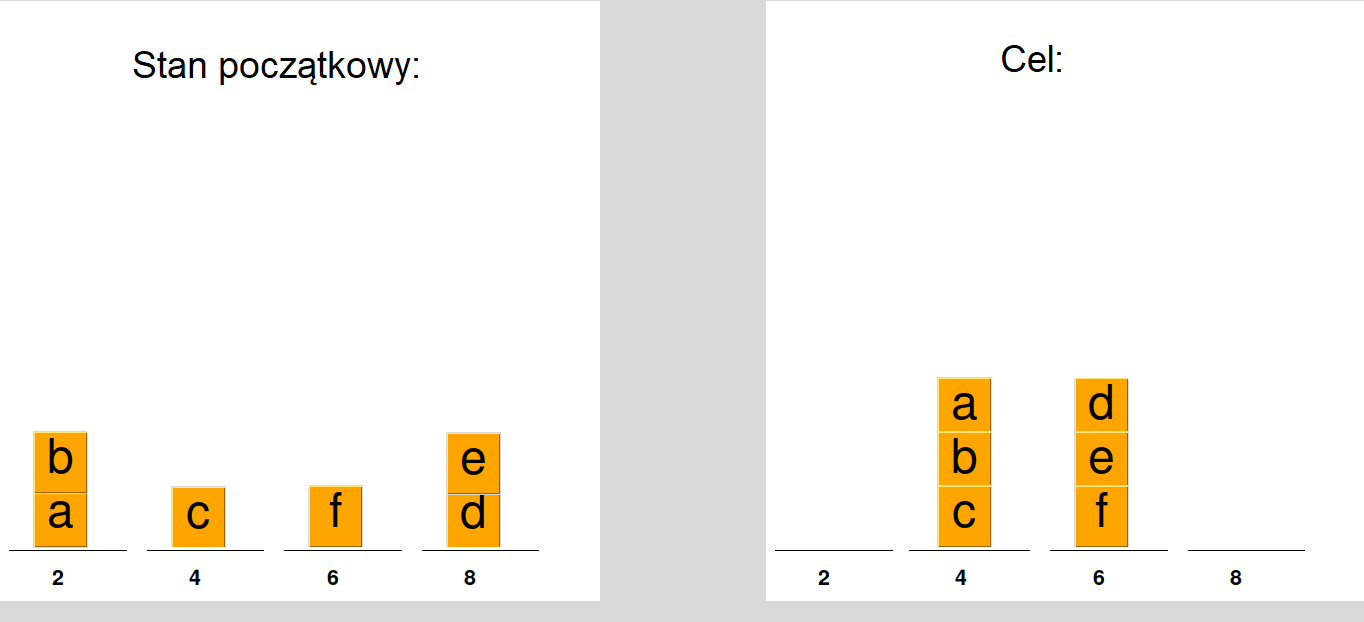
\includegraphics[scale=0.45]{RownolegleTest1}
        \centering
        \caption{Przyklad łamigłówki z użytym mechanizmem równoległości}
        \label{Conc}
    \end{figure}
    Drugi przykład polega na przemieszczaniu się robotów w przestrzeni.
    \begin{figure}[H]
        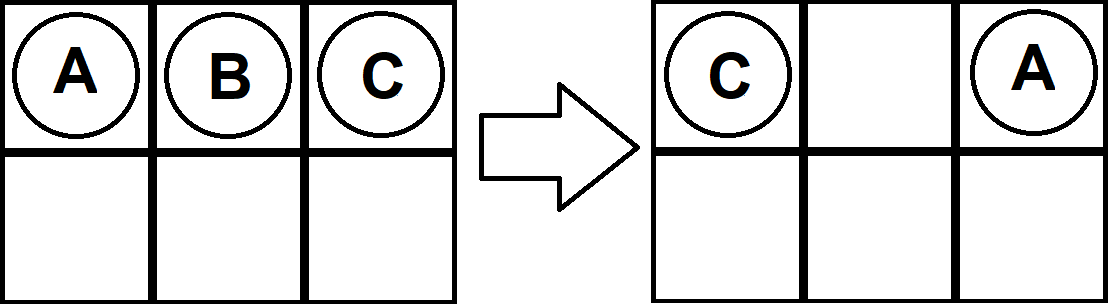
\includegraphics[scale=0.5]{RownolegleTest2}
        \centering
        \caption{Stan początkowy oraz cel dla przemieszczania}
        \label{Swaps}
    \end{figure}
    Zgodnie z przyjętą konwencją numerowanie kafelków odbywa się rzędami od lewej do prawej. To, co należy zauważyć to fakt, iż wyspecyfikowane cele 
    nie muszą zawierać informacji o wszystkich obiektach. To może mieć znaczenie w sytuacjach, w których użytkownik przez przypadek zdefiniuje 
    cel dla obiektu, którego poprawne ułożenie w świecie jest zbędne, \\
    a znacznie spowolni pracę algorytmu.
    \subsection{Wyniki}
    Przyglądając się obrazkowi \ref{Conc} łatwo zauważyć, iż zaprezentowany problem można podzielić na dwa identyczne podproblemy, gdyż sytuacja przedstawiona 
    w świecie jest symetryczna. Dodatkowo cele również posiadają taką własność. Po uruchomieniu algorytmu dla zadanego przypadku otrzymano
    nastepujący rezultat
    \begin{figure}[H]
        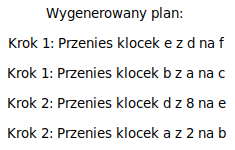
\includegraphics[scale=0.9]{PrzykladRownolegloscPlan}
        \centering
        \caption{Wygenerowany plan dla sytuacji \ref{Conc}}
    \end{figure}
    Zgodnie z przewidywaniami, algorytm skonstruował odpowiedni plan w dwóch krokach, w każdym z nich wykonując po dwie operacje
    
    \begin{figure}[H]
        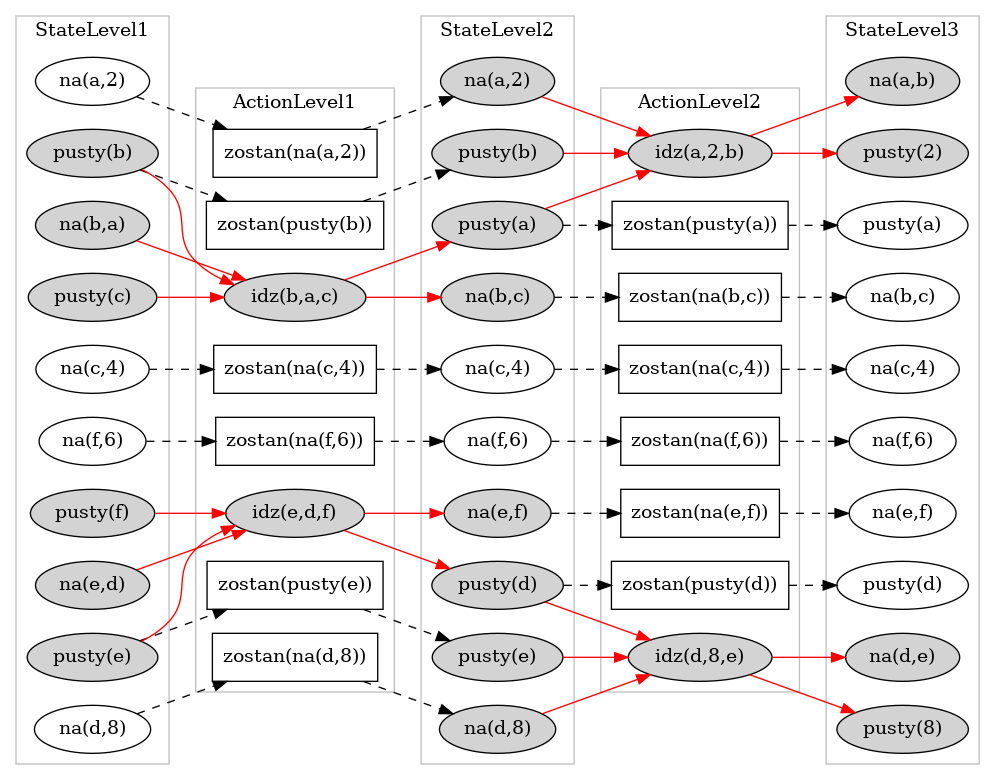
\includegraphics[scale=0.4]{RownolegloscSimplePlan}
        \centering
        \caption{Graf prosty przedstawiajacy rozwiązanie problemu \ref{Conc}}
    \end{figure}

    Dla drugiego przykładu również udało się utworzyć, nieco bardziej skomplikowany, plan działania:

    \begin{figure}[H]
        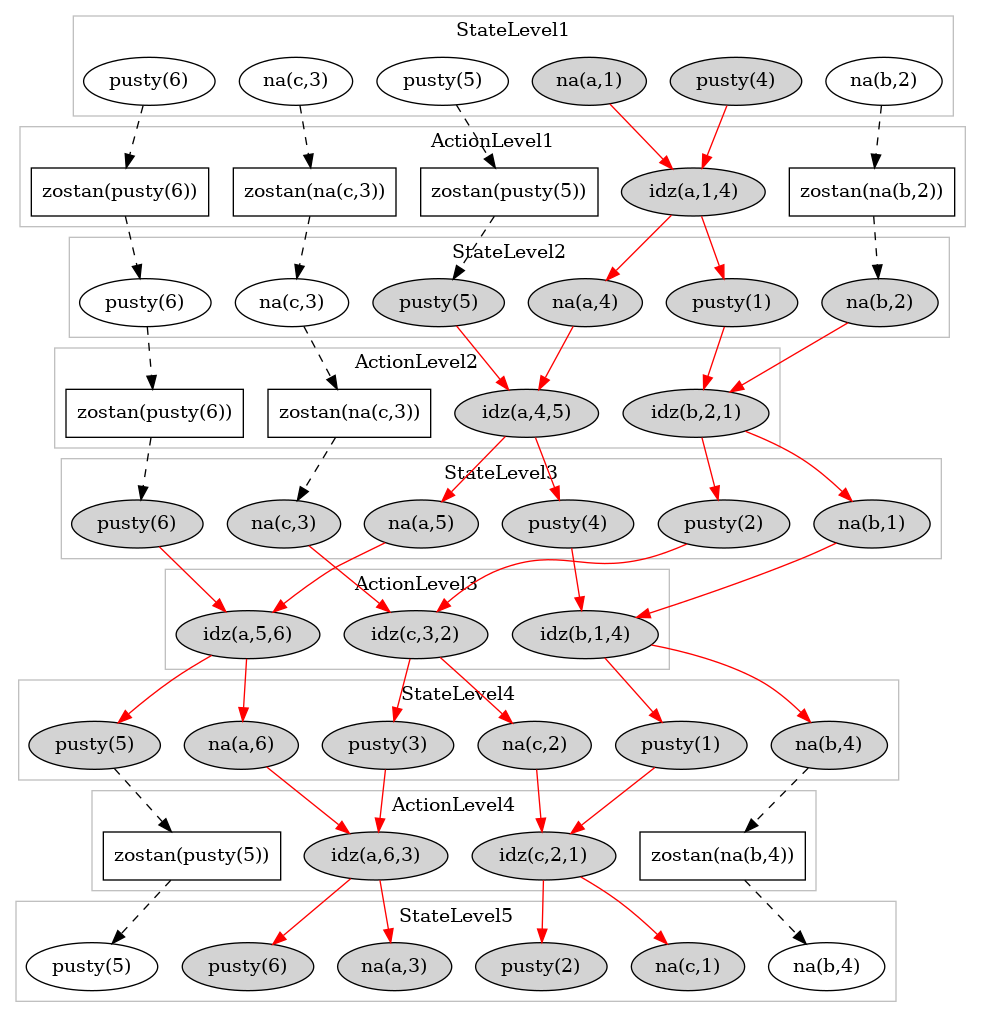
\includegraphics[scale=0.4]{RownolegloscSimple2}
        \centering
        \caption{Graf prosty przedstawiajacy rozwiązanie problemu \ref{Swaps}}
    \end{figure}



    \subsection{Wnioski}
    Mechanizm rownoległości jest klarownie widoczny na grafach prostych. Analizując utworzone struktury dla planów równoległych należy zauważyć, iż 
    w żadnym wypadku strzałki zaznaczone kolorem czerwonym nie generują niespójnych efektów.
    Przedstawiona implementacja GRAPHPLAN'u, zgodnie z jego założeniami, potrafi generować plany równoległe, które nie powodują niespójności 
    na żadnym etapie transformacji świata. W sytuacji, w której użytkownik dysponuje możliwością jednoczesnego dokonania większej liczby operacji
    niż jedna, GRAPHPLAN zdecydowanie przewyższa metody wykorzystujące mechanizmy planowania liniowego.
%\section{Przemieszczanie w przestrzeni}
%    \subsection{Wprowadzenie}
%    \subsection{Przykład}
%    \subsection{Szczegóły implementacyjne}
%    \subsection{Wyniki}
%    \subsection{Wnioski}
%\section{Wieża Hanoi}
%    \subsection{Wprowadzenie}
%    \subsection{Przykład}
%    \subsection{Szczegóły implementacyjne}
%    \subsection{Wyniki}
%    \subsection{Wnioski}
%\section{Osiem Hetmanów}
%\label{OsiemHetmanowTest}
%    \subsection{Wprowadzenie}
%    \subsection{Przykład}
%    \subsection{Szczegóły implementacyjne}
%    \subsection{Wyniki}
%    \subsection{Wnioski}